\documentclass[11pt]{article}
% Horizontal Magnetic Dipole over a lossy half-space
\usepackage[utf8]{inputenc} % Use it to include other characters than ABC
\usepackage[cmex10]{amsmath}
\usepackage{mdwmath}
\usepackage{mdwtab}
\usepackage{hyperref}
\usepackage{physics} % For using the oridnary derivative nomenclature
\usepackage{datetime} % Insert date and time
\usepackage[letterpaper, margin=1in]{geometry}
\usepackage{graphicx}
% \usepackage{mathptmx} % Times new Roman

% ------------------------------- Useful Tricks Learnt
% Use ={}& to align subequations to the left
% Use = for single equations
%
% ----------------- To compile with references use the following order in Shell"
% 1. pdflatex filename.tex
% 2. bibtex filename (no extension)
% 3. bibtex filename (no extension)
% 4. pdflatex filename.tex
% -----------------

\begin{document}
  \title{\textsc{Integral Formulation of a Horizontally Oriented Magnetic Dipole in a layered medium}\\}
  \date{\footnote{Last Modified: \currenttime, \today.}}
  \maketitle

  We model the current distribution in a two-dimensional electron gas (2DEG) at a GaN/AlGaN heterostructure with a horizontal magnetic dipole (HMD) embedded in a layered medium as illustrated in Fig.\ref{fig:illustration}.

  \begin{figure}[h]
    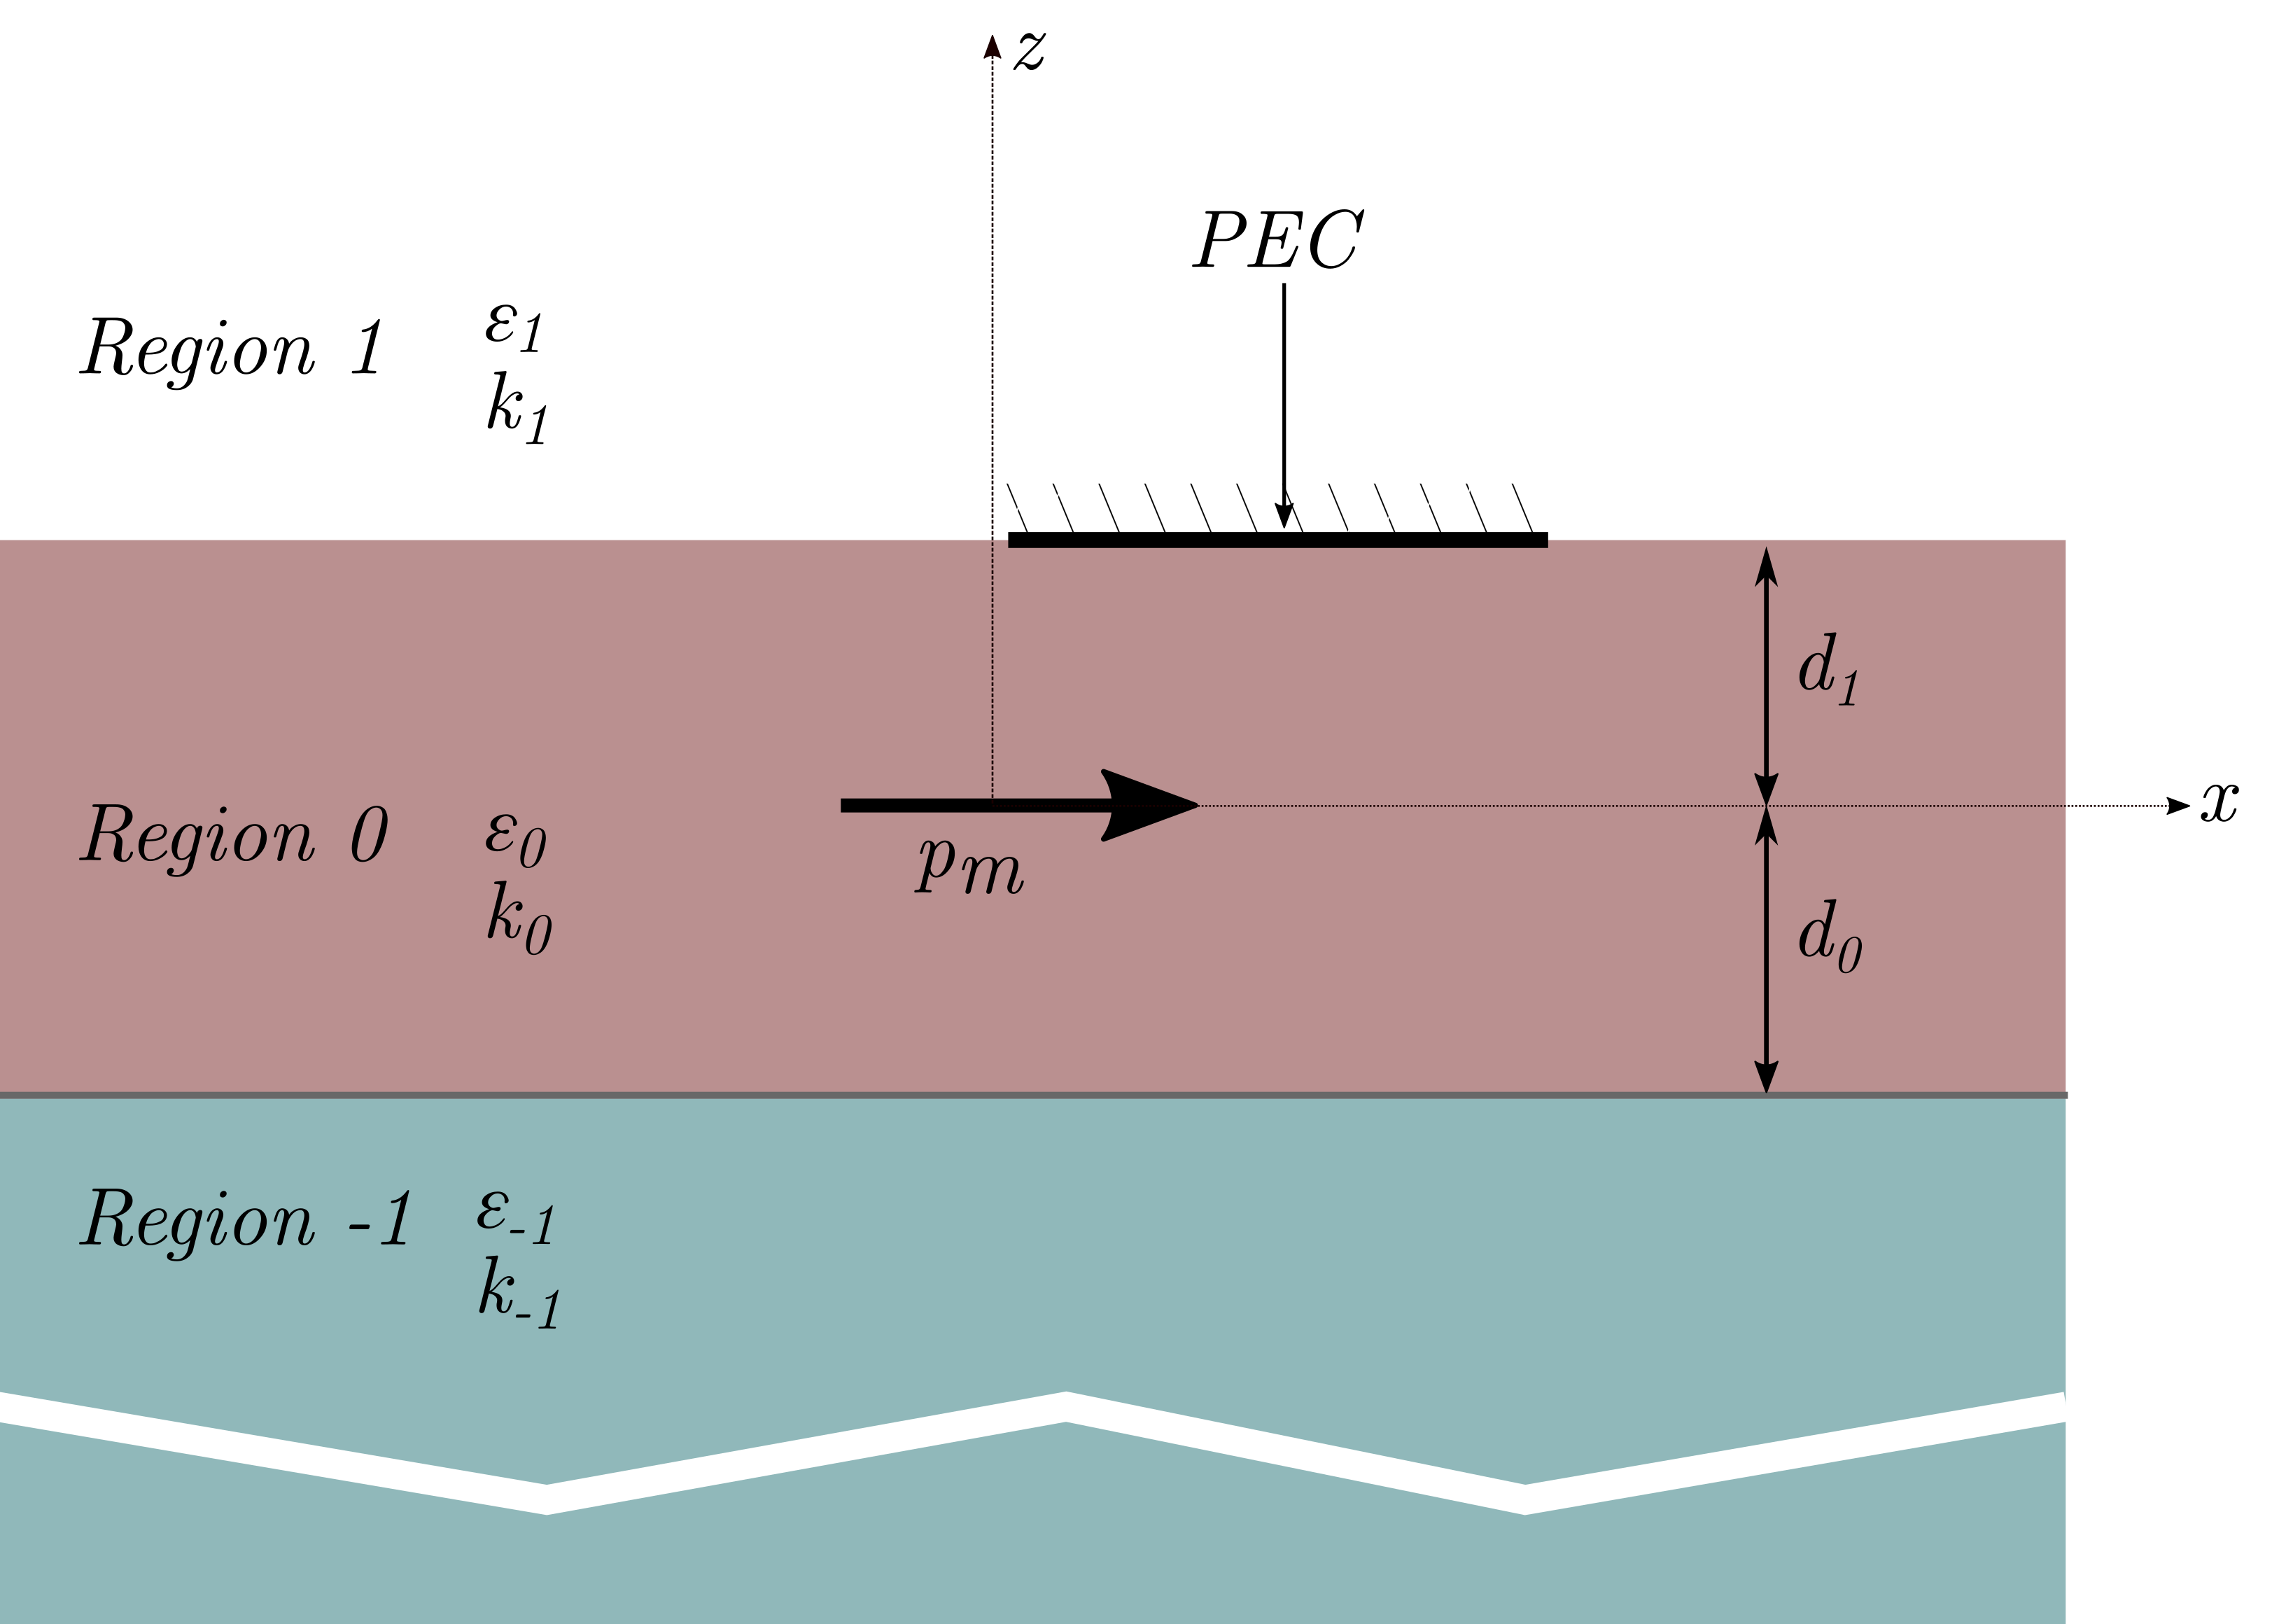
\includegraphics[width=12cm]{Gated_2DEG_structure}
    \centering
    \caption{Three layer Structure}
    \label{fig:illustration}
  \end{figure}
  
  \section{Green's Function Formulation}

  We consider a stratified medium with three layers with the dipole placed at the origin and the layered labeled as $0$ with dielectric constant $\varepsilon_0$, different from the free-space permittivity. We consider two semi-infinite layers, above (Region 1) at $z=d_1$ and below (Region -1) the source layer at $z=d_0$ that extend to infinity. Assuming a TM case, the fields can be described by the electric field longitudinal component, $E_z$,
  \begin{equation}
    E_z = \int_{-\infty}^{\infty} E_z(\rho) dk_{\rho}
    \label{eq:Ez}
  \end{equation}

  In region $i$, the $E_z$ field can be written as:

  \begin{equation}
    E_z^i = \int_{-\infty}^{\infty} \left[ A_i e^{j k_{z_i}z} + B_i e^{-j k_{z_i}z} \right] H_n^{(1)}(k_{\rho}\rho) C_n(\phi) dk_{\rho}
    \label{eq:TM_Ez}
  \end{equation}

  where, $H_n^{(1)}(k_{\rho}\rho)$ is the nth-order Hankel function of the first kind and $C_n(\phi)$ is $\phi$ based function depending on the order of Hankel function and the dipole configuration. The remaining electric and magnetic field components can be found by the following Maxwell's equations:

  \begin{subequations}
    \begin{align}
      E_{\rho} =  \frac{1}{k_{\rho}^2} \frac{\partial}{\partial \rho} \frac{\partial E_z(k_\rho)}{\partial z}
      \label{eq:E_rho} \\
      E_{\phi} =  \frac{1}{k_{\rho}^2} \frac{1}{\rho} \frac{\partial}{ \partial \phi} \frac{\partial E_z(k_\rho)}{\partial z}
      \label{eq:E_phi}
    \end{align}
    \label{eq:E_fields}
  \end{subequations}

  \begin{subequations}
    \begin{align}
      H_{\rho} = -\frac{j\omega \varepsilon_i}{k_{\rho}^2} \frac{1}{\rho}\frac{\partial E_z(k_\rho)}{\partial \phi}
      \label{eq:H_rho} \\
      H_{\phi} =  +\frac{j\omega \varepsilon_i}{k_{\rho}^2} \frac{1}{\rho} \frac{\partial E_z(k_\rho)}{\partial \rho}
      \label{eq:H_phi}
    \end{align}
    \label{eq:H_fields}
  \end{subequations}

  The unknowns $A_i$ and $B_i$ can be found by applying boundary conditions at the two interfaces at $z = d_1$ and $z=d_0$ that require the continuity of tangential components of the electric and magnetic fields. From (\ref{eq:TM_Ez}), (\ref{eq:E_rho}) and (\ref{eq:H_rho}), we obtain:

  \begin{equation}
    k_{z_i} \left( A_i e^{jk_{z_i} d_i} - B_i e^{-jk_{z_i} d_i}  \right) = k_{z_{i-1}} \left( A_{i-1} e^{jk_{z_{i-1}} d_i} - B_{i-1} e^{-jk_{z_{i-1}} d_i}  \right)
    \label{eq:E_rho_BC}
  \end{equation}

  \begin{equation}
    \varepsilon_i \left( A_i e^{jk_{z_i} d_i} - B_i e^{-jk_{z_i} d_i}  \right) = \varepsilon_{i-1} \left( A_{i-1} e^{jk_{z_{i-1}} d_i} - B_{i-1} e^{-jk_{z_{i-1}} d_i}  \right)
    \label{eq:H_rho_BC}
  \end{equation}

  In the region 0, the position of the observation point above or below the source leads to different values of unknowns $A_0$ and $B_0$. To make it distinct, for $z>0$,the unknowns are written as $A^>$ and $B^>$ and for $z<0$, $A^<$ and $B^<$ respectively. For HMD, the following conditions are used.\cite{kong1990electromagnetic}

  \begin{subequations}
    \begin{align}
      A_0^> = A_{hmd} + E_{hmd} \\
      A_0^< = A_{hmd}
      \label{eq:A_0} \\
      B_0^> = B_{hmd} \\
      B_0^< = B_{hmd} + E_{hmd}
      \label{eq:B_0}
    \end{align}
    \label{eq:hmd}
  \end{subequations}

  where,
  \begin{equation}
    E_{hmd} = \frac{p_m \omega \mu_0 k_{\rho}^2}{8 \pi k_{0z}}
    \label{eq:E_hmd}
  \end{equation}

  \begin{equation}
    H_{hmd} = -\frac{p_m k_{\rho}^2}{8 \pi}
    \label{eq:H_hmd}
  \end{equation}

  where $p_m$ is the dipole moment of the current source. The longitudinal propagation constant in region $i$ is given by:
  \begin{equation}
    k_z^i = \sqrt{k_i^2 - k_{\rho}^2}
    \label{eq:k}
  \end{equation}

  Now using (\ref{eq:E_rho_BC}) and (\ref{eq:H_rho_BC}), at $z=d_1$, we have:
  \begin{equation}
    k_{z_1} \left( A_1 e^{jk_{z_1} d_1} - B_1 e^{-jk_{z_1} d_1}  \right) = k_{z_0} \left( A_{0}^> e^{jk_{z_0} d_1} - B_{0}^> e^{-jk_{z_0} d_1}  \right)
    \label{eq:E_rho_d1}
  \end{equation}

  \begin{equation}
    \varepsilon_1 \left( A_1 e^{jk_{z_1} d_1} - B_1 e^{-jk_{z_1} d_1}  \right) = \varepsilon_{0} \left( A_{0}^> e^{jk_{z_0} d_1} - B_{0}^> e^{-jk_{z_0} d_1}  \right)
    \label{eq:H_rho_d1}
  \end{equation}

  By adding (\ref{eq:E_rho_d1}) and (\ref{eq:H_rho_d1}) we get:
  \begin{equation}
    \left( k_{z_1} + \varepsilon_1 \right) A_1 e^{jk_{z_1} d_1} - \left( k_{z_1} - \varepsilon_1 \right) B_1 e^{-jk_{z_1} d_1}  = \left( k_{z_0} + \varepsilon_0 \right) A_0^> e^{jk_{z_0} d_1} - \left( k_{z_0} - \varepsilon_0 \right) B_0^> e^{-jk_{z_0} d_1}
    \label{eq:sum}
  \end{equation}

  The unknowns $A_1$ and $B_1$ can be expressed in terms of $A_0^>$ and $B_0^>$ as \cite{kong1990electromagnetic}:
  \begin{equation}
    A_1 e^{jk_{z_1} d_1} = \frac{1}{2} \left[ \frac{\varepsilon_0}{\varepsilon_1} + \frac{k_{z_0}}{k_{z_1}} \right] \times \left[  A_0^> e^{jk_{z_0} d_1} + R^{\uparrow} B_0^> e^{-jk_{z_0} d_1} \right]
    \label{eq:A_1}
  \end{equation}

  \begin{equation}
    B_1 e^{-jk_{z_1} d_1} = \frac{1}{2} \left[ \frac{\varepsilon_0}{\varepsilon_1} + \frac{k_{z_0}}{k_{z_1}} \right] \times \left[R^{\uparrow}  A_0^> e^{jk_{z_0} d_1} + B_0^> e^{-jk_{z_0} d_1} \right]
    \label{eq:B_1}
  \end{equation}

  where, $R^{\uparrow}$ is the TM Fresnel reflection coefficient at $ z=d_1$ as seen from region 0,
  \begin{equation}
    R^{\uparrow} = \frac{-\varepsilon_0 k_{z_1} + \varepsilon_1 k_{z_0}}{\varepsilon^0 k_{z_1} + \varepsilon^1 k_{z_0}}
    \label{eq:R_up}
  \end{equation}

  Through a similar procedure by applying boundary conditions at $z=d_{-1}$, coefficients $A_{-1}$ and $B_{-1}$ are obtained:
  \begin{equation}
    A_{-1} e^{jk_{z_{-1}} d_{0}} = \frac{1}{2} \left[ \frac{\varepsilon_0}{\varepsilon_{-1}} + \frac{k_{z_0}}{k_{z_{-1}}} \right] \times \left[  A_0^< e^{jk_z{z_{-1}} d_0} + R^{\downarrow} B_0^< e^{-jk_{z_{-1}} d_0} \right]
    \label{eq:A_-1}
  \end{equation}

  \begin{equation}
    B_{-1} e^{-jk_{z_{-1}} d_0} = \frac{1}{2} \left[ \frac{\varepsilon_0}{\varepsilon_{-1}} + \frac{k_{z_0}}{k_{z_{-1}}} \right] \times \left[R^{\downarrow}  A_0^< e^{jk_{z_{-1}} d_0} + B_0^< e^{-jk_{z_{-1}} d_0} \right]
    \label{eq:B_-1}
  \end{equation}
  where, $R^{\downarrow}$ is the TM Fresnel reflection coefficient at $ z=d_0$ as seen from region 0,
  \begin{equation}
    R^{\downarrow} = \frac{-\varepsilon_0 k_{z_{-1}} + \varepsilon_{-1} k_{z_0}}{\varepsilon_0 k_{z_{-1}} + \varepsilon_{-1} k_{z_0}}
    \label{eq:R_up}
  \end{equation}

  For a structure having three regions, it is observed that $B_1$ and $A_{-1}$ equals zero due to the open nature of region 1 and -1 respectively. By manipulating (\ref{eq:E_rho_d1}) and (\ref{eq:H_rho_d1}), we obtain the reflection coefficient in region 0 at $z=d_1$:

  \begin{equation}
    \Gamma_0^{\uparrow} = \frac{B_0^>}{A_0^>} = +\frac{e^{j2k_{z_0} d_1}}{R^{\uparrow}} + \frac{ \left[ 1 - (1/{R^{\uparrow}}^2) \right]e^{j2(k_{z_0} + k_{z_1}) d_1}}{(1/R^{\uparrow})e^{j2k_{z_1} d_1}}
    \label{eq:gamma_up}
  \end{equation}

  Similarly, the reflection coefficient in region 0 at $z=d_0$ is given by:
  \begin{equation}
    \Gamma_0^{\downarrow} = \frac{A_0^<}{B_0^<} = +\frac{e^{-j2k_{z_0} d_0}}{R^{\downarrow}} + \frac{ \left[ 1 - (1/{R^{\downarrow}}^2) \right]e^{-j2(k_{z_0} + k_{z_{-1}}) d_0}}{(1/R^{\downarrow})e^{-j2k_{z_{-1}} d_0}}
    \label{eq:gamma_down}
  \end{equation}

  From (\ref{eq:H_hmd}),(\ref{eq:gamma_up}) and (\ref{eq:gamma_down}), we obtain:
  \begin{equation}
    \Gamma_0^{\downarrow} = \frac{A_0^<}{B_0^<} = +\frac{e^{-j2k_{z_0} d_0}}{R^{\downarrow}} + \frac{ \left[ 1 - (1/{R^{\downarrow}}^2) \right]e^{-j2(k_{z_0} + k_{z_{-1}}) d_0}}{(1/R^{\downarrow})e^{-j2k_{z_{-1}} d_0}}
    \label{eq:gamma_down}
  \end{equation}

  \begin{subequations}
    \begin{align}
      \Gamma_0^{\uparrow} = \frac{B_0^>}{A_0^>} = \frac{B_{hmd}}{A_{hmd} + E_{hmd}}
      \label{eq:gamma_0_up} \\
      \Gamma_0^{\downarrow} = \frac{A_0^<}{B_0^<} = \frac{A_{hmd}}{B_{hmd} + E_{hmd}}
      \label{eq:gamma_0_down}
    \end{align}
    \label{eq:gammas}
  \end{subequations}

  The coefficients in region 0, therefore can be written as:
  \begin{subequations}
    \begin{align}
      A_0^> = \frac{1 + \Gamma_0^{\downarrow}}{1- \Gamma_0^{\uparrow} \Gamma_0^{\downarrow}} E_{hmd}
      \label{eq:A0up} \\
      B_0^> = \frac{\Gamma_0^{\uparrow}(1 + \Gamma_0^{\downarrow})}{1- \Gamma_0^{\uparrow} \Gamma_0^{\downarrow}} E_{hmd}
      \label{eq:B0up} \\
      A_0^< = \frac{\Gamma_0^{\uparrow}(1 + \Gamma_0^{\uparrow})}{1- \Gamma_0^{\uparrow} \Gamma_0^{\downarrow}} E_{hmd}
      \label{eq:A0up} \\
      B_0^> = \frac{1 + \Gamma_0^{\uparrow}}{1- \Gamma_0^{\uparrow} \Gamma_0^{\downarrow}} E_{hmd}
      \label{eq:B0up} \\
    \end{align}
    \label{eq:coefficients}
  \end{subequations}

  Once the electric field in region 0 is found  using (\ref{eq:TM_Ez}) and (\ref{eq:coefficients}), fields in other regions can be found using Eqs. (\ref{eq:A_1})-(\ref{eq:B_-1}).

  \subsection{Gated Region}

  A perfect electric conductor (PEC) is placed at the interface of region 0 and 1 at $z=d_1$. The Fresnel reflection coefficient (\ref{eq:R_up}) reduces to $-1$ in this case.



  \bibliography{mylib}
  \bibliographystyle{ieeetr}
\end{document}
